% \documentclass[a4paper, 9pt, fleqn]{diss}
% \include{format-and-defs}
% \begin{document}

%%%%%%%%%%%%%%%%%%%%%%%%%%%%%%%%%%%%
\chapter{Semantic processing}
\label{s:german-locative-phrases-semantic-processing}

In previous sections, I concentrated on how to represent the semantics
of spatial relations. In this section I focus on how to conceptualize, 
i.e. how to choose a particular spatial relation, frame of 
reference, landmark or perspective in order to refer to some object
in the environment. This chapter gives an overview of the factors
influencing conceptualization (\sectref{s:factors-of-conceptualization}),
followed by details of how conceptualization for spatial scenes can
be implemented (\sectref{sec:8.2}). Lastly, I compare the approach favored in this
book to another approach often used in modeling 
(\sectref{s:categorization+discrimination}). This last 
section also looks at the performance of the conceptualization
machinery presented in this chapter.


\section{Factors influencing semantic processing}
\label{s:factors-of-conceptualization}
A number of factors influencing the particular
choice in a particular context have been identified by scholars. 
First, the communicative intention of the speaker plays a major role. 
Whether the speaker wants to describe the spatial position of an 
object or discriminate it with respect to other objects in the context or whether
he is trying to give a route description \citep{tversky1998space}\oldindex{Tversky, B.}\oldindex{Lee, P.},
impacts on which spatial relations agents choose to express.
Second, the context and in particular the presence and position of landmarks,
their affordances with respect to frames of reference, the presence
of geocentric reference systems and the perspective of the interlocutor 
all influence the choices agents make.
Third, the available repertoire of spatial relations, frames of reference,
as well as cultural factors are no less important. For instance, in some cultures 
social status governs the choice of perspective.
How to talk about an object, in other words, how to conceptualize
the world for reaching the particular communicative goal
technically requires agents to choose semantic structure, 
including semantic operations and categories. 
Since we understand semantic structure as a program, the process 
of choosing appropriate semantic structure is essentially one of 
automatic programming, in which programs are constructed and 
tested based on their fitness for the particular task. 
The fitness or utility of some automatically constructed semantic structure 
is decided based on (1) the current communicative goal, e.g. to discriminate an object, 
(2) current spatial setup, in particular the position of objects,
(3) available categories and concepts.


\begin{figure}
\begin{centering}
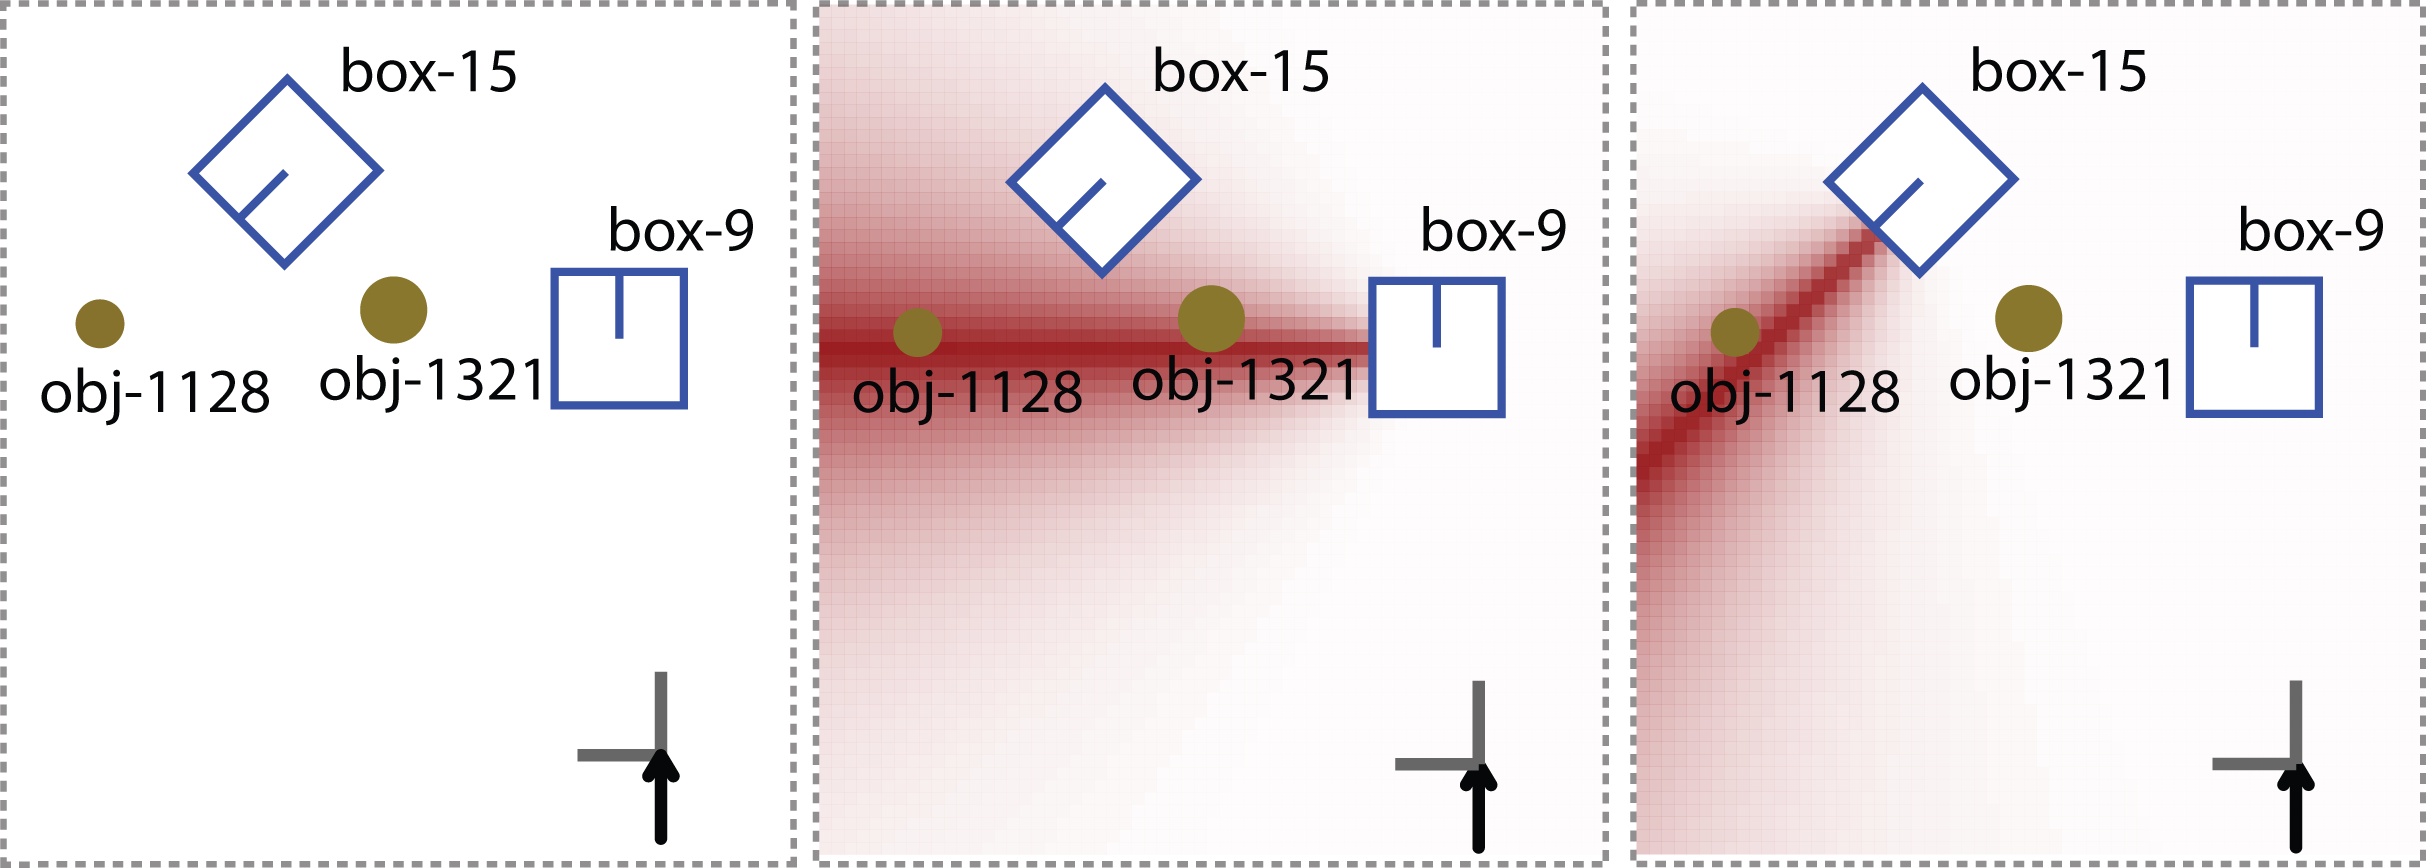
\includegraphics[width=.8\columnwidth]{figs/description-vs-discrimination.png}
\end{centering}
\caption[Difference between discrimination and description]
{Difference between description and discrimination. The left figure
shows the original context. The middle picture shows that
object {\footnotesize\tt obj-1128} lies in the region described by ``left of box-9'' 
(intrinsic reading) with a high score. However, object {\footnotesize\tt obj-1321}
lies pretty much in the same region of high applicability. In other words,
``left of box-9'' is not discriminating. The right figure shows an example of
a discriminating spatial relation. ``In front of box-15'' (intrinsic reading) 
clearly discriminates object {\footnotesize\tt obj-1128} from {\footnotesize\tt obj-1321},
as the score of both objects for this description varies significantly.}
\label{f:discrimination-vs-description}
\end{figure}

% communicative goal
\subsection{Influence of type of communicative goal -- which vs where}
Which communicative goal an agent is pursuing is an important 
driving factor in how he will conceptualize the world for reaching 
that goal. But it is not only the particular object an agent wants to talk 
about that makes a difference, but also the agent's intentions with 
respect to the object. For instance, there are important differences 
between descriptive and discriminating utterances. 
In discrimination scenarios, in answers to questions 
of the form \textit{Welcher?} (`which') the hearer is required to distinguish, in 
other words identify, an object. This relies chiefly on the overall 
spatial setup including the position of other objects 
in the scene. \textit{Wo?} (`where') questions, e.g. \textit{Wo ist der Block?} (`where is the block'),  
on the other hand are asking for descriptions of the spatial relations an object takes 
part in. In psychological experiments
spatial descriptions are elicited using contexts with only a 
single object \citep{levinson2003space}\oldindex{Levinson, S. C.}. 
In description scenarios the applicability
of a spatial relation is the important aspect, 
whereas in discrimination scenarios, the power to contrast the
target object from the rest of the objects is more important 
(\citealt{tenbrink2005identifying}\oldindex{Tenbrink, T.}, see \figref{f:discrimination-vs-description} for an example). 
Agents in discrimination scenarios choose spatial relations and
reference systems based on maximizing the distance to other objects
\citep{herskovits1986language}\oldindex{Herskovits, A.}.

\subsection{Influence of spatial contexts}
Naturally, the spatial position of objects in the context has a
direct effect on which spatial relations might be applicable for
discriminating an object. This is based on
the discussion of discrimination in the previous paragraph, 
but it also holds, somewhat trivially, because the position of an 
object with respect to another object determines the applicability 
of a spatial relation between the two. But there are of course other factors
related to context that need to be taken into account.
Examples are the presence or absence of landmarks for construing the world
in relation to them and the availability of geocentric
features which allow for the application of absolute frames of 
reference. Furthermore, landmarks without intrinsic features, such 
as trees who have no inherent front, 
prevent the application of intrinsic frames of reference, and lastly, available perspectives on a scene influence the layout
of relative frames of reference on landmarks. In other words,
the particular spatial setup has an effect on the 
space of possible or even desirable conceptualizations.

\begin{figure}
\begin{centering}
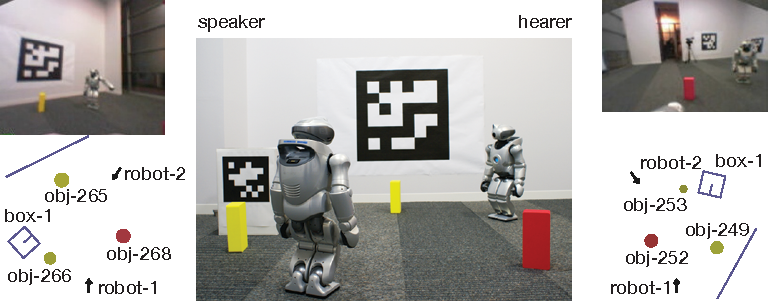
\includegraphics[width=.8\columnwidth]{figs/space-scene-2-small}
\end{centering}
\caption[Spatial setup example]
{Spatial setup}
\label{f:space-scene-2}
\end{figure}

\begin{figure}
\begin{centering}
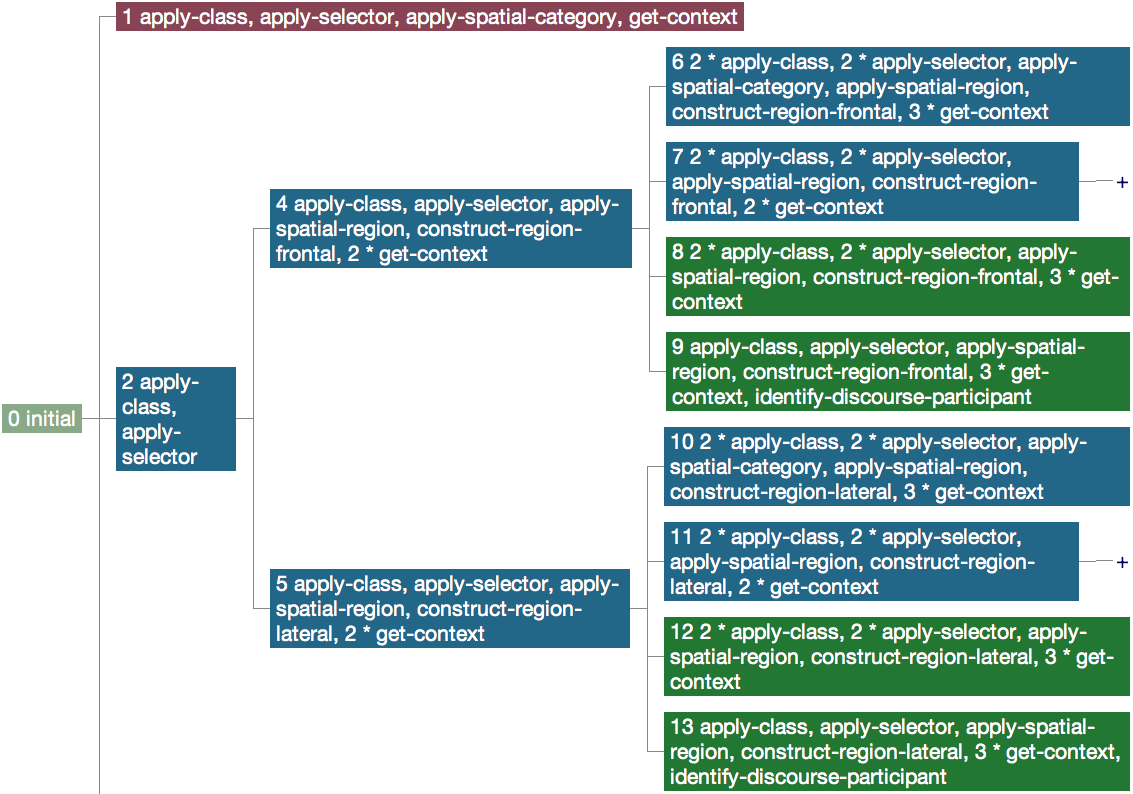
\includegraphics[width=1\columnwidth]{figs/conceptualization.png}
\end{centering}
\caption[Example search tree for conceptualization of a spatial scene.]
{Part of the conceptualization search tree for the spatial scene depicted
in \figref{f:space-scene-2}.
Some conceptualizations are rejected (red node), because they do not work
from the perspective of the hearer. This semantic structure in the red node 
in this figure corresponds to a determined spatial adjective noun phrase 
which is rejected because of the different
perspectives of the two robots on the scene. Green nodes 
show successful conceptualizations. In total around 30 conceptualizations 
for the topic are found which differ in degree of
applicability; some of them are more applicable than others.}
\label{f:conceptualization-search}
\end{figure}

\begin{figure}
\begin{centering}
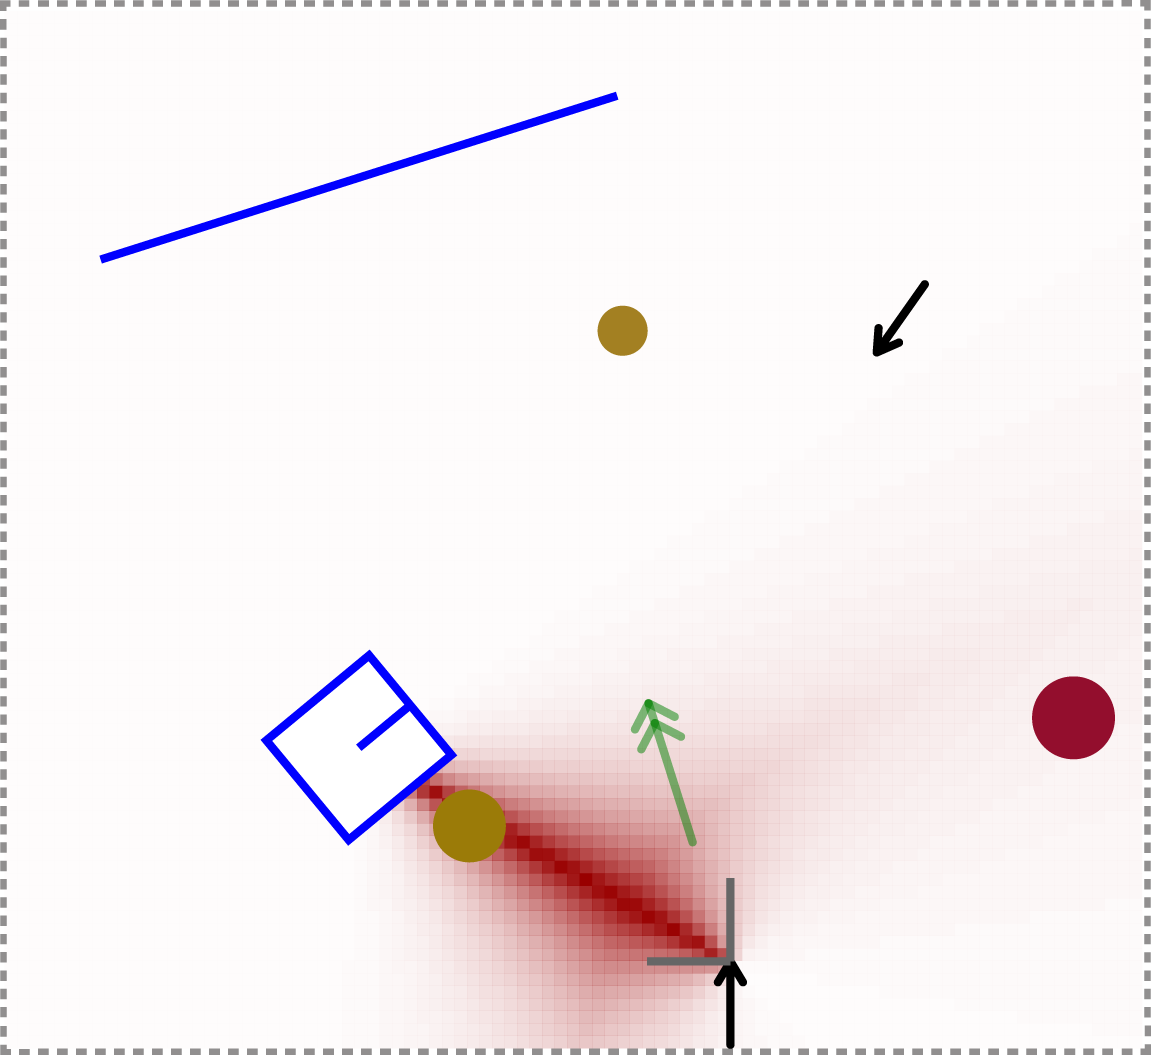
\includegraphics[width=0.25\columnwidth]{figs/conceptualization-in-front-of-the-box-from-my-perspective-region.png}
% \hspace{1pt}
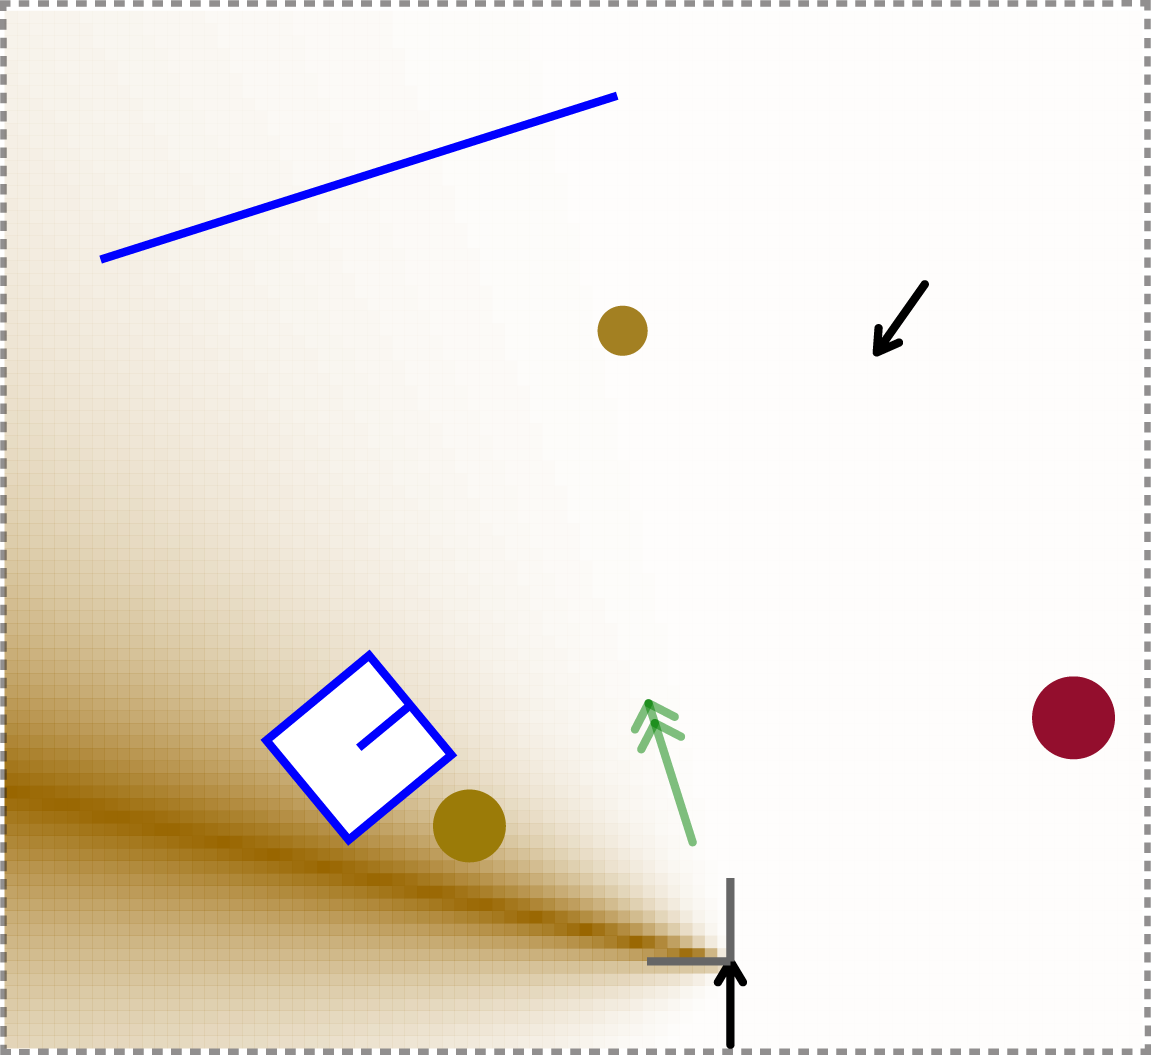
\includegraphics[width=0.25\columnwidth]{figs/conceptualization-right-of-me-from-your-perspective-region.png}
% \hspace{1pt}
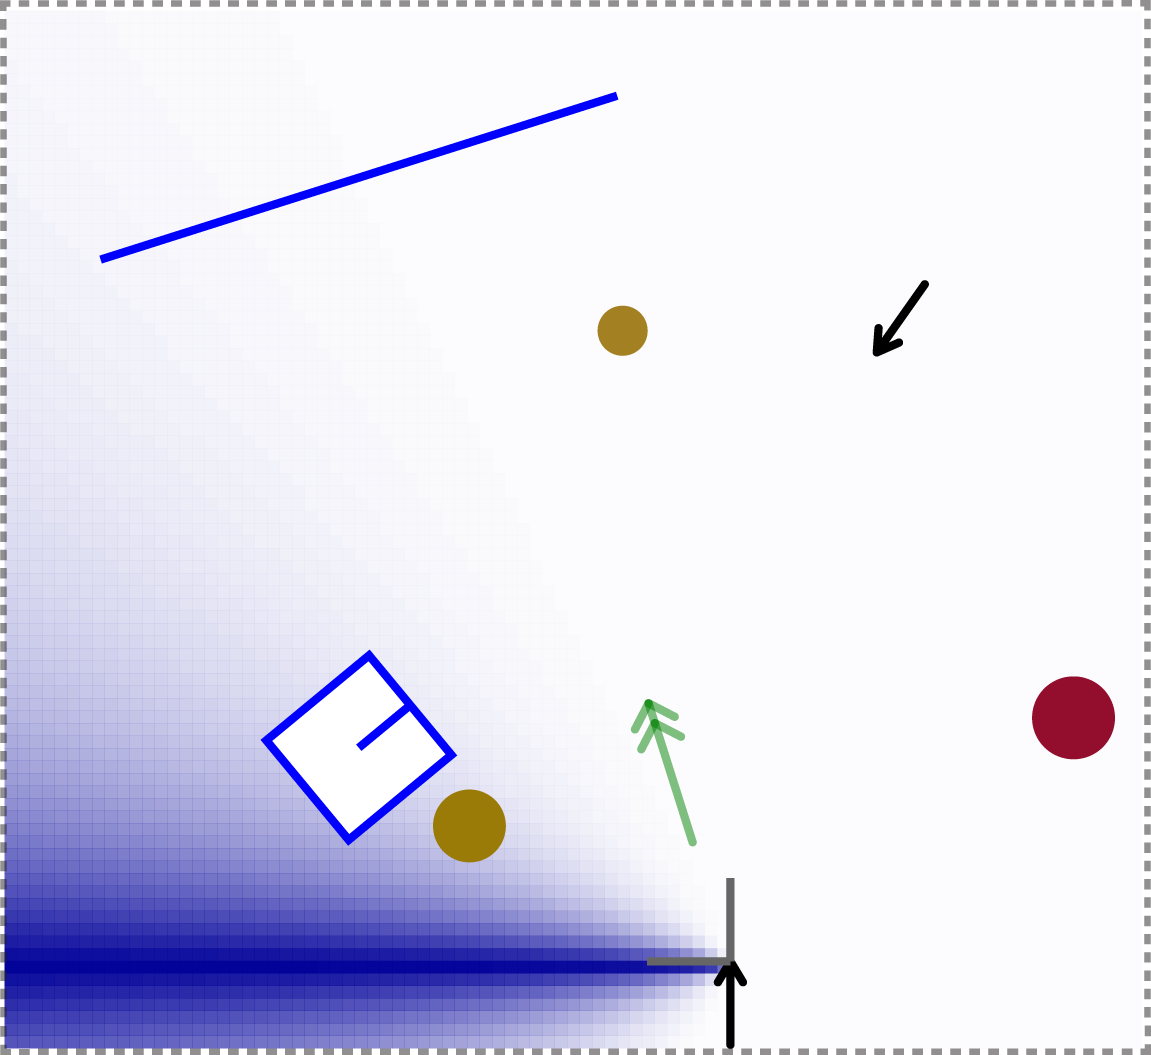
\includegraphics[width=0.25\columnwidth]{figs/conceptualization-left-of-me-region.png} \\
\vspace{1.5pt}
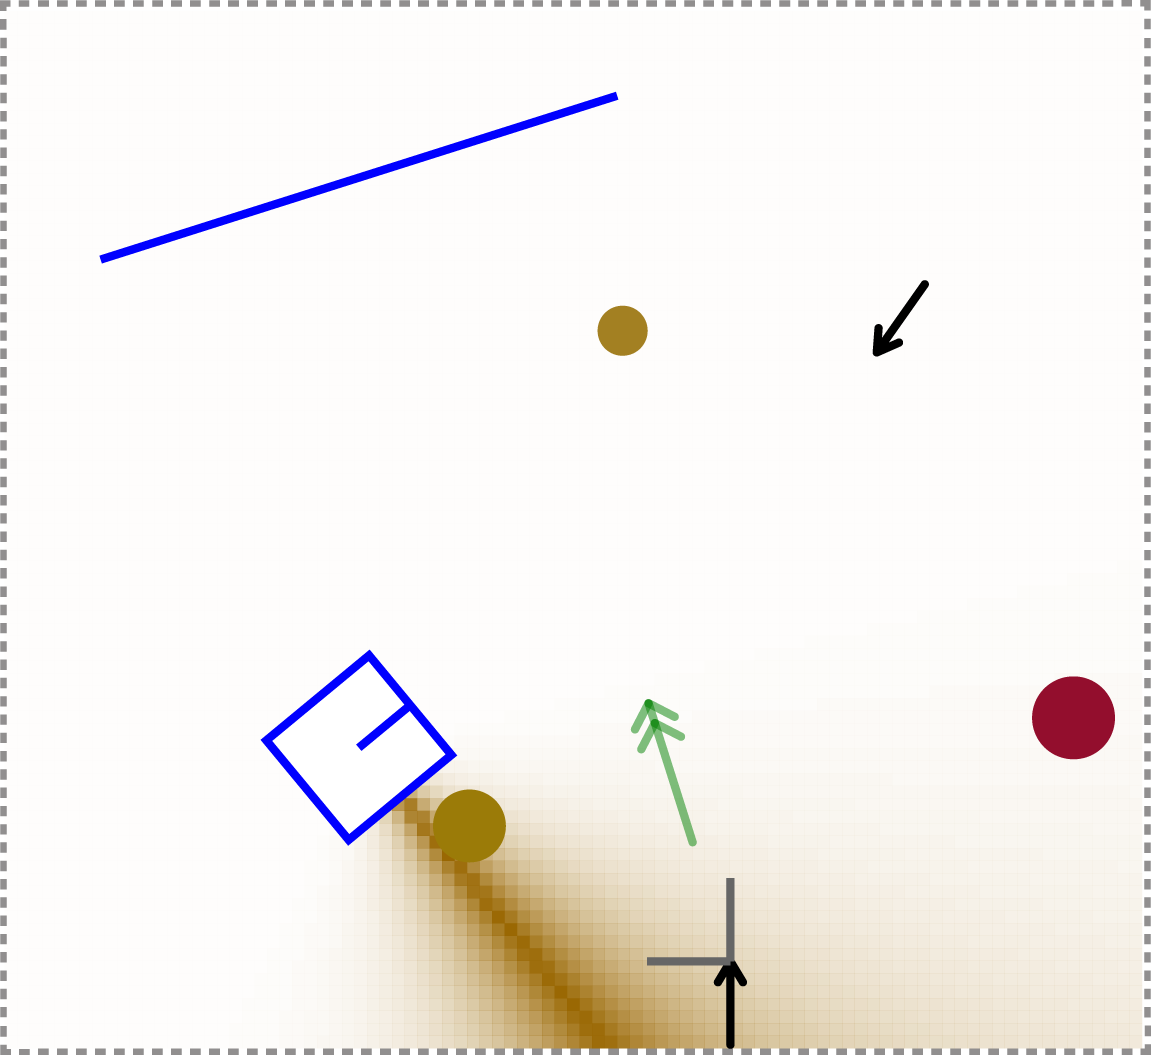
\includegraphics[width=0.25\columnwidth]{figs/conceptualization-right-of-the-box-region.png}
% \hspace{1pt}
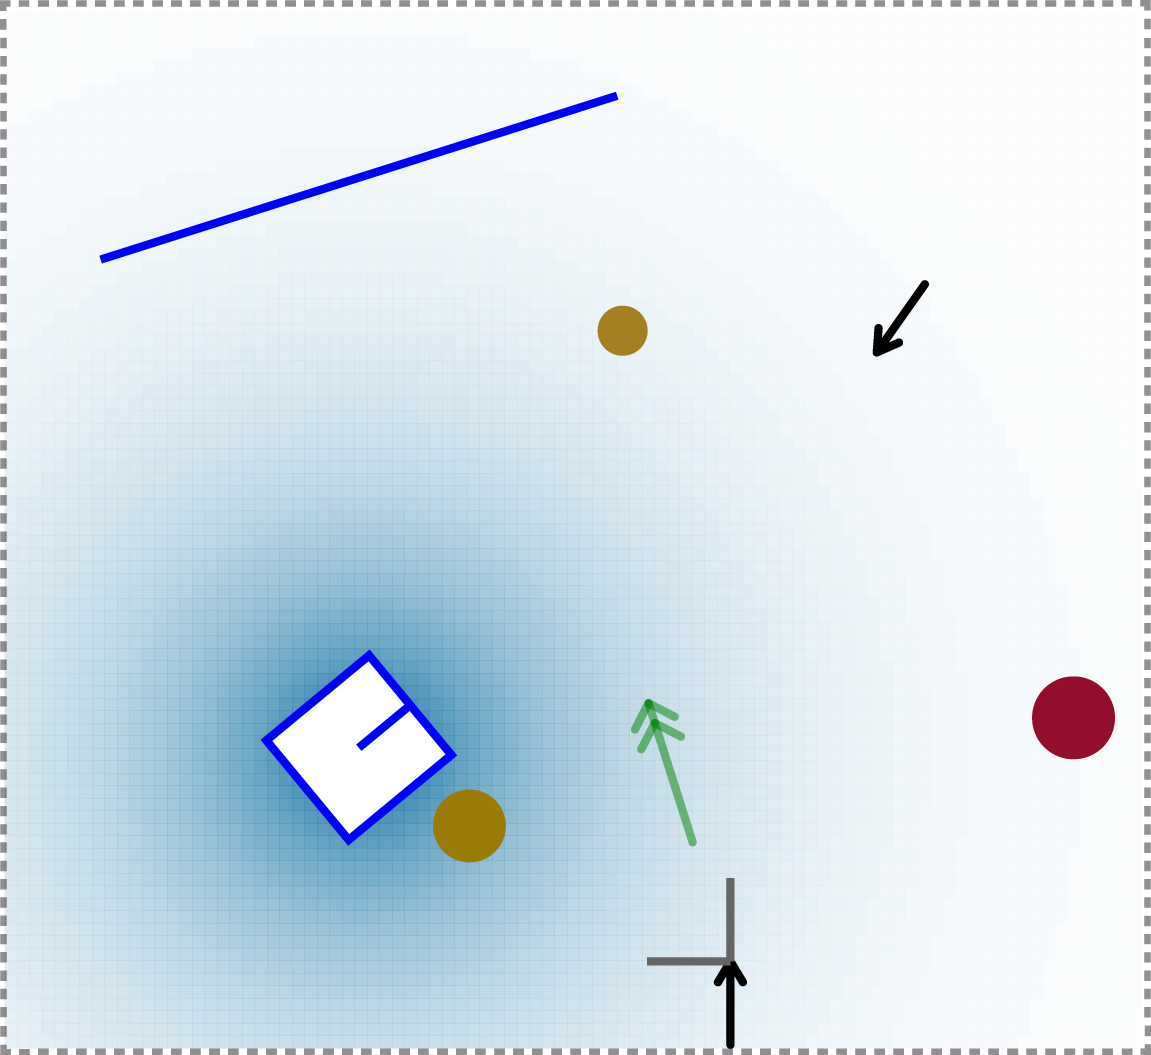
\includegraphics[width=0.25\columnwidth]{figs/conceptualization-near-the-box-region.png}
% \hspace{1pt}
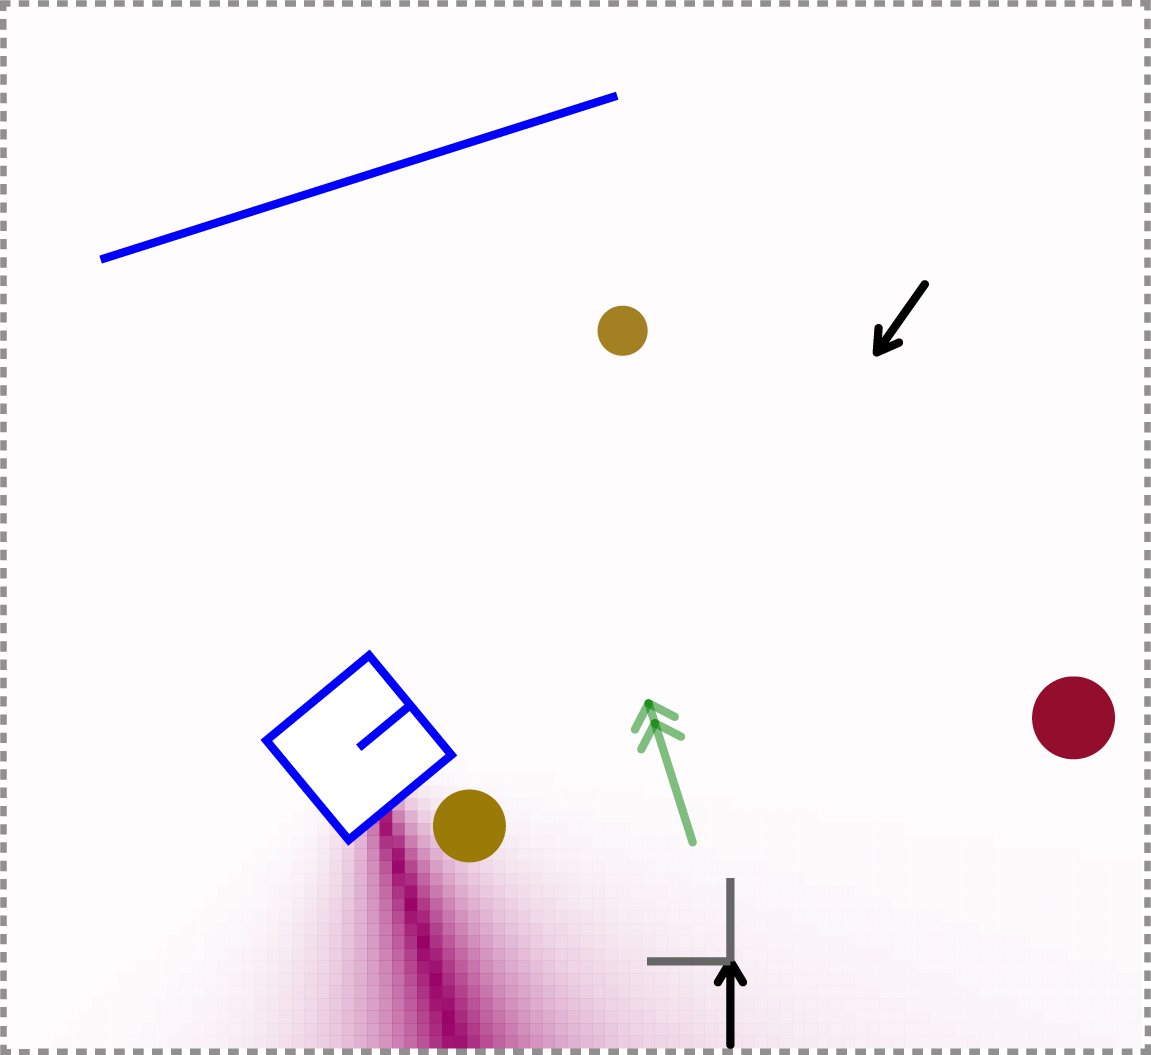
\includegraphics[width=0.25\columnwidth]{figs/conceptualization-south-of-the-box-from-my-perspective-region.png}

\caption[Conceptualization examples]
{The search process in \figref{f:conceptualization-search} finds more than
30 different conceptualizations for object {\footnotesize\tt obj-266} 
in the spatial scene depicted in \figref{f:space-scene-2}.
Some of them are depicted here in terms of regions that are 
described by the them. From left top to bottom right the figure
shows the regions used to discriminate the target object. In the
following, roughly corresponding utterances and discrimination scores
for the particular semantic structure are shown.\\
\begin{tabularx}{\linewidth}{r@{~}c@{~}>{\raggedright\arraybackslash}X}
0.55 & -- & \textit{der Block vor der Box von mir aus} \newline(`the block in front of the box')\\
0.50 & -- & \textit{der Block rechts von mir von dir aus} \newline(`the block right of me from your perspective')\\
0.38 & -- & \textit{der Block links von mir} (`the block left of me')\\
0.36 & -- & \textit{der Block rechts der Box} (`the block right of the box')\\
0.30 & -- & \textit{der Block nahe der Box} (`the block near the box')\\
0.23 & -- & \textit{der Block s\"udlich der Box} (`the block south of the box')
\end{tabularx}}
\label{f:conceptualization-results}
\end{centering}
\end{figure}

\section{Implementing spatial conceptualization}\label{sec:8.2}
Implementing the conceptualization of spatial scenes is based on 
two computational steps. Semantic structure is, first, automatically
combined and, second, it is ranked based on the particular
communicative goal. We use a search algorithm 
(see \chapref{s:irl}) as a means to 
automatically combine simple semantic building blocks 
into more complex ones. Semantic structure assembled in the search process is 
immediately tried on the current context, given the specific 
target object and rated based on how well it fulfills the communicative goal. 

\subsection{Ranking of semantic structure}
The scoring of semantic structure is guided by the communicative goal 
of the agent. For discrimination tasks, for example, the score of a particular 
semantic structure is mainly determined by how 
big the overall similarity of the target object is in contrast to 
the score of all other objects in the context. 
The \textsc{discrimination score} \is{discrimination score}
$\operatorname{disc}$ for the object $o$ with respect to other
objects $O$ is computed by subtracting the maximum
of all scores of the objects $o'$ in $O$ from the score $s_o$ of $o$.
\begin{eqnarray}
\operatorname{disc}_{o,O}=s_o - \max_{o' \in O}s_{o'}
\end{eqnarray}
The discrimination score is computed by evaluating the 
particular semantic structure whose discrimination score 
is to be determined and more specifically by evaluating the semantic operation 
{\footnotesize\tt apply-selector}. This operation singles out objects 
from sets of objects by choosing the object with the highest
similarity score and binding it with its discrimination score 
$\operatorname{disc_{o_{target},O}}$. 
For scoring semantic structure only the discrimination
score of the target object of the semantic structure is
of importance (see \figref{f:disc-score} for an example 
of accumulating similarities over a semantic structure).

\begin{figure}
\begin{center}
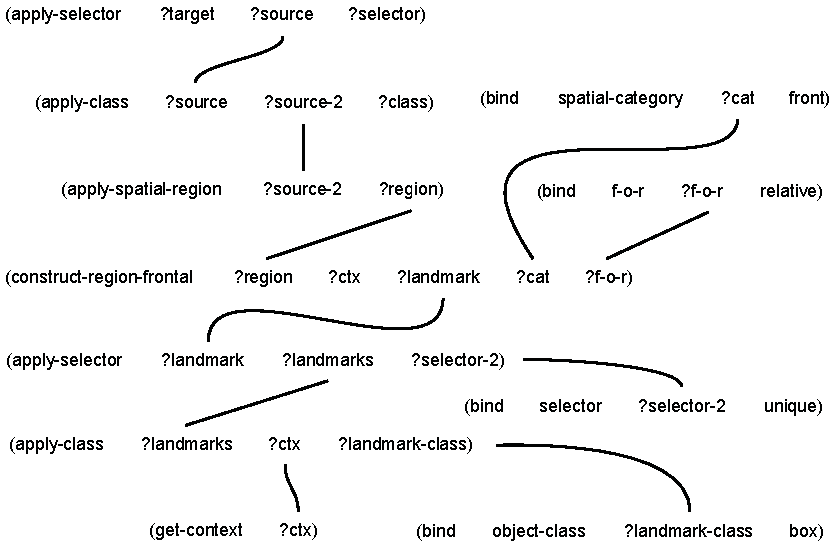
\includegraphics[width=0.8\columnwidth]{figs/semantic-structure-in-front-of-the-box-relative}
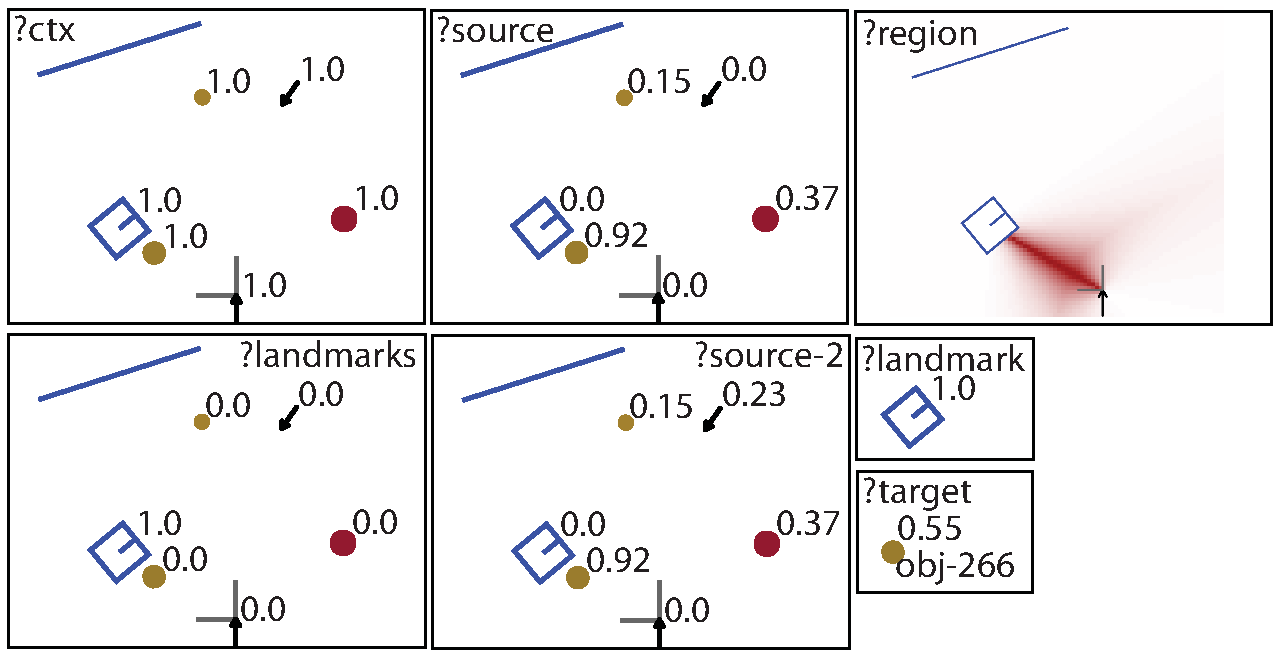
\includegraphics[width=0.8\columnwidth]{figs/semantic-structure-in-front-of-the-box-relative-evaluation}
\end{center}
\caption[Evaluation of semantic structure and discrimination scores]{%
Evaluation of semantic structure and discrimination scores. The top figure 
shows a semantic structure which is evaluated.
The bottom shows the bindings of variables resulting from evaluation. 
Objects have scores, and their scores are tracked and multiplied, which leads from the
context where every object has a score of $1.0$ to categorized sets such as the one
bound to {\footnotesize\tt ?landmarks} where the object class {\footnotesize\tt box} has been applied which 
results in all objects having a score of $0.0$ except for the box. Similarly, the region is applied
({\footnotesize\tt ?source-2}), followed by the application of the object class {\footnotesize\tt block}
({\footnotesize\tt ?source}). Finally, the topic ({\footnotesize\tt ?target}) is identified.}
\label{f:disc-score}
\end{figure}

Besides the discrimination score, other factors can be incorporated
into ranking semantic structure. For instance, one can include
the scores of categories and semantic entities, whether or not 
the semantic structure also would work if applied from the perspective
of the hearer, etc. The following is a non-exhaustive
list of the factors that can be included into ranking semantic
structure.

\begin{figure}
\begin{center}
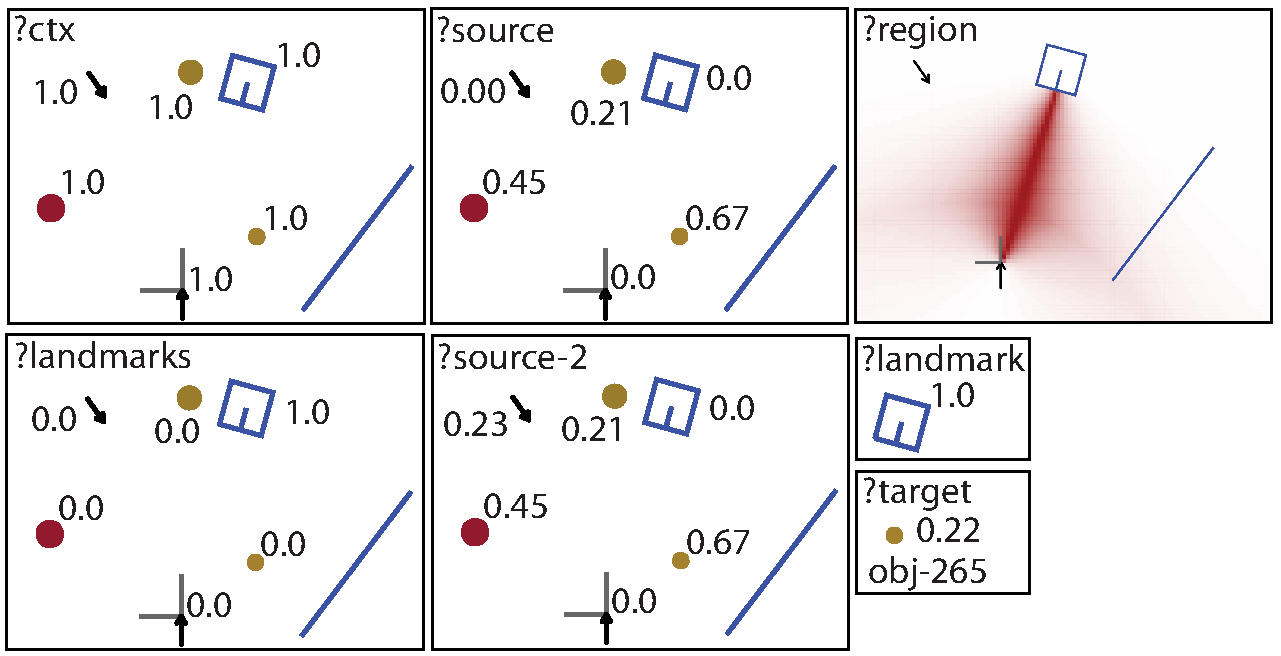
\includegraphics[width=.8\columnwidth]{figs/semantic-structure-in-front-of-the-box-relative-evaluation-prediction-hearer}
\end{center}
\caption[Predictive evaluation from the perspective of the hearer]
{Predictive evaluation of the semantic structure shown in \figref{f:disc-score}. The speaker can test semantic structure how he thinks it 
would get evaluated by the hearer. In the case of the semantic structure shown
in \figref{f:disc-score} (top) the result of evaluation is object {\footnotesize\tt obj-265},
which is different from the target of the semantic structure when evaluated
from the perspective of the speaker (then it was object {\footnotesize\tt obj-266}).
In some sense this structure is ambiguous as to which object it refers to,
since the semantic structure is not explicitly perspective-marked.
On the other hand, the discrimination score of object {\footnotesize\tt obj-266} 
from the perspective of the
speaker is much higher ($0.55$) than the score for object {\footnotesize\tt obj-265} 
from the perspective of the hearer. In other words, if this would indeed be
the perspective of the hearer and not just a prediction, the agent could
choose to interpret {\footnotesize\tt obj-265} to be the target object.}
\label{f:predictiv-evaluation}
\end{figure}

\begin{description}
\item[Score of categories and semantic entities]
Categories and semantic entities such as frames of reference can be 
scored to reflect how 
conventional a particular item is. This allows to model preferences for
certain categories as, for instance, English native speakers show
preference for lateral over frontal categories, but also allows to 
capture \citep{tversky1999speakers}\oldindex{Tversky, B.}\oldindex{Lee, P.}\oldindex{Mainwaring, S.} preferences for certain 
frames of reference. English speakers, for instance, 
have been observed to prefer the relative frame of reference
over the intrinsic one \citep{levinson2003space}\oldindex{Levinson, S. C.},
and German speaker seem to prefer the intrinsic over the relative frame of reference 
\citep{ehrich1985linguistik}\oldindex{Ehrich, V.}. Although evidence for these kinds of phenomena
seems at least contradictory (see \citealt{miller1976language}\oldindex{Johnson-Laird, P. N.}\oldindex{Miller, G. A.} for 
reverse findings for English speakers) nevertheless the assumption
that one frame of reference is conventionally selected more often 
is reasonable and can be incorporated into the 
scoring of semantic structure.
\item[Score of chunks]
Chunks -- the building blocks of semantic structure -- are themselves scored entities.
The score of chunks reflects how conventional or preferred a 
particular way of conceptualizing reality is. Languages, for instance, and their
syntactic regularities clearly reflect certain preferred conceptual choices. For instance,
in Russian, verbs always feature lexical Aktionsarten which conceptualize every event
in a way that highlights a particular aspect of that event, e.g. the beginning or the end or
that it repeats, etc. The syntactic need to express
these distinctions points to conceptualization strategies that are required to
build correct Russian sentences. Such strategies can easily be expressed with chunks
and their preference by scoring them accordingly \citep{gerasymova2010acquisition}\oldindex{Gerasymova, K.}\oldindex{Spranger, M.}.\is{measures!conceptualization strategy similarity}
\item[Perspective Choice]
In many situations speakers seem to prefer to conceptualize
reality from the perspective of the hearer. Social status and
cognitive abilities of the hearer \citep{mainwaring2003descriptions}\oldindex{Ohgishi, M}\oldindex{Tversky, B.}\oldindex{Mainwaring, S.}\oldindex{Schiano, D.}, 
as well as politeness \citep{schober1993spatial}\oldindex{Schober, M. F.} 
and the question who is required to act \citep{tversky2009perspective}\oldindex{Tversky, B.}\oldindex{Hard, B. M.}
all have been observed to affect choice of perspective. Typically this
entails that the perspective of the addressee or hearer is preferred over
the perspective of the speaker. Choice of perspective is relevant for 
two cases of semantic structure. First, it is relevant for  
dealing with relative frames of reference and landmarks as in adverbial
and prepositional phrases in which the perspective on the scene 
overtly controls the way the scene is conceptualized. 
The other one is less obvious and relates to semantic structures that 
covertly depends on perspective such as 
group-based reference systems. In principle there are two ways 
to incorporate perspective into the ranking of semantic structure both of 
which rely on the fact that the speaker immediately tries semantic
structure from the perspective of the hearer. The first one is to outwardly
reject semantic structure that does not evaluate to the desired 
target object when evaluated from the perspective of the hearer or any
other desired perspective (see \figref{f:predictiv-evaluation} 
for an example of such a case). 
The other, more subtle one, is to compute the discrimination score
of the semantic structure from the perspective of the hearer. In other words,
while by default every agent uses his own perspective on the context
to score semantic structure, the robot now uses the perspective of the interlocutor.
To transform the context to the perspective of the hearer, each robot
continuously tracks the position of the interlocutor and subsequently
can use this information to evaluate semantic structure as he
predicts the interlocutor would execute the structure. Of course,
this is only a prediction in the sense that the speaker has
no certainty about the position of the interlocutor in the spatial
setup. Nevertheless, this is a hugely powerful device that
can eliminate many misunderstandings in communication 
before they occur. It is important to realize that in many situations
the choice of perspective has no or negligible effects
which is mainly true for contexts where 
the perspectives of the interlocutors overlap sufficiently.
Humans in such cases also do not mark perspective 
\citep{tenbrink2005dimensional}\oldindex{Tenbrink, T.}.
Additionally, there are ways to even out the effect
of perspective by explicitly marking the perspective in the semantic
structure using the perspective transform operation
{\footnotesize\tt geometric-transform}. Such semantic structure
behaves like intrinsic or absolute spatial relations, since
the perspective is part of the structure. For spatial
adjectives this kind of marking of perspective
seems to be impossible in the sense that it cannot be conveyed
in language. In such cases a joint strategy by speaker
and hearer, for instance, the choice to always conceptualize from
the perspective of the hearer can be beneficial.

\item[Length of semantic structure]
Speakers thrive to be efficient in how
they communicate \citep{dale1995computational}\oldindex{Dale, R.}\oldindex{Reiter, E.}. The longer the 
semantic structure is for
discriminating a particular target object, the more needs to
be expressed in language. Length of semantic structure thus 
can be an important influence on the scoring of semantic structure.
Typically long semantic structures are punished.
\end{description}

These and other influences are easily incorporated 
into the scoring function of semantic structure which is the crucial
ingredient ultimately deciding which semantic structures from the vast space
of possible semantic structures are worth considering. 
The other important ingredient in implementing conceptualization 
is governing how semantic structure is assembled in the first place.
This process is one of automatic programming in which
chunks of semantic structure are combined based on 
input-output arguments. Figures~\ref{f:conceptualization-search} 
and~\ref{f:conceptualization-results} show the conceptualization 
search tree and some results of conceptualizing semantic 
structure for object {\footnotesize\tt obj-266} 
in the spatial scene depicted in \figref{f:space-scene-2}.

%\subsection{Additional Influences on Conceptualization not incorporated}
%discourse -> easily incorporated, however here no discourse
%representation

%%%%%%%%%%%%%%%%%%%%%%%%%%%%%%%%%%%%
\subsection{Ready-made semantic structure}
The size of chunks used in the conceptualization search process 
has a considerable influence on how elaborate
the search process in conceptualization has to be in order to find suitable
semantic structure for the particular communicative goal an agent might have.
In order to handle the large space of conceptualization, chunks can 
reflect various degrees of ready-made semantic structure with some 
being very large covering complete utterances such as determined spatial
adjective noun phrases, to smaller building blocks. How to choose 
the particular layout of chunks from the standpoint of designing
a running system is a decision that depends on how flexible the system
needs to be.


%%%%%%%%%%%%%%%%%%%%%%%%%%%%%%%%%%%%
\section{Categorization and discrimination}
\label{s:categorization+discrimination}
An important part of the complete machinery for discriminating an object
in the environment is the problem of how spatial categories and relations
themselves are applied. In computational modeling, discrimination is often conflated with categorization,
or to be more precise, with a certain approach to categorization which can 
be called \textsc{strict category membership}\is{categorization!strict} (see \citealt{belpaeme2007language}\oldindex{Bleys, J.}\oldindex{Belpaeme, T.} 
for an application of this approach to color). Categorization is understood here
as strict membership in which a point in the sensorimotor 
space is categorized as belonging
to the one category closest to him. For instance, an 
object is considered to be red, when red is the color category 
that is most similar to it. If this is the case the object is a member
of the red category. Consequently, every point in the sensorimotor space 
belongs to precisely one category of the set of categories and the
complete sensorimotor space can be decomposed 
into different sets of objects based on their category membership, 
a process known as Voronoi tesselation (\citealt{aurenhammer1991voronoi}\oldindex{Aurenhammer, F.}, see \figref{f:voronoi}).
Applying such an approach to discrimination, one needs to additionally 
define some criteria as to when a category $c$ can be called discriminating
object $o$ from the context $O$. The strict category membership approach
posits two requirements to be met.
\begin{description}
\item[Strict membership] $o$ is said to be a strict member of the category $c$, iff
 $o$ is closer to $c$ than to any other category from the repertoire of categories $C$.
 In order for $c$ to be called to discriminate $o$, $o$ has to be a strict member of $c$.
\item[Discriminating category] In order for $c$ to be discriminatory,
$o$ has to be the only object from the context $O$ that is a strict member of the category
$c$.
\end{description}
Of course, the first criteria is a necessary condition for the second to apply,
but in terms of objections that I will discuss following this approach, 
it makes sense to consider both of them separately. 

There are two lines of arguments why such an approach to discrimination
is wrong. First, there is accumulating evidence from natural language that
is in conflict with both criteria. For instance, many scholars propose
alternative principles particularly in conflict with the discriminating 
category criteria. Rather then requiring $c$ to be the only category 
closest to $o$, they require that $o$ is the closest object to $c$ 
without further constraining the other objects in $O$ and their relationship
to $c$. So other objects in $O$ can be strict members of $c$ as long as they
are not closer to $c$ than $o$. In fact what seems to be driving
people in their choice of categories in discrimination task seems to be most
importantly the principle of \textsc{greatest distance} or greatest 
contrast \is{greatest distance principle}\is{greatest contrast|see{greatest distance principle}} 
which only requires the category to establish sufficient difference
between the distance of object $o$ and all other objects in the context.
Such principles have been used generally to explain peoples behavior in 
object discrimination tasks \citep{hermann1976objektbenennung}\oldindex{Hermann, T.}\oldindex{Grabowski, J.}
and also have been applied more specifically to spatial language 
(see the \textsc{shifting contrast principle} \is{shifting contrast principle|see{greatest distance principle}}introduced by 
\citealt{herskovits1986language}\oldindex{Herskovits, A.} and similar ideas in \citealt{freksa1999links}\oldindex{Freksa, C.}).
These insights primarily relate to criterion two. But one can also use them 
to attack the strict membership criterion. If humans really
are looking for categories that establish high contrast, the assumption
that $o$ has to be closest to the category $c$ in order for $c$ to be
even considered clearly has to be wrong. For instance, $c$ might not
be the category that is closest to $o$, however, if it establishes enough 
contrast between $o$ and all other objects in the context it does not 
have to be. This seems to be the case for spatial language. 
\cite{tenbrink2005identifying}\oldindex{Tenbrink, T.}, for instance, found that unmodified 
projective terms are frequently used by participants in a discrimination task
for referring to objects that are far away from the prototypical axes. Now clearly
in such tasks the linguistic material available to natural language speakers 
allows them to be much more precise about the actual spatial position
in the sense claimed to be relevant by the strict membership criterion.
In other words, speakers could choose to describe a spatial relation 
for objects based on smallest distance to some prototypical point, but they
choose not to. So there seems to be some empirical evidence that
speakers behave differently than claimed by these two principles.

The second line of arguments against the strict category membership 
approach to discrimination comes from computational modeling. In particular, we
can compare the approach advocated in this book with the strict category membership \oldindex{strict category membership|see{categorization!strict}}
to discrimination and show that it performs better
in real-world scenarios. To be able to compare the two approaches
we obviously need an implementation of both. I have already sketched
the approach in the previous chapters, and I will sketch the implementational
details of the strict category membership approach in the following paragraphs.

\begin{figure}
\begin{center}
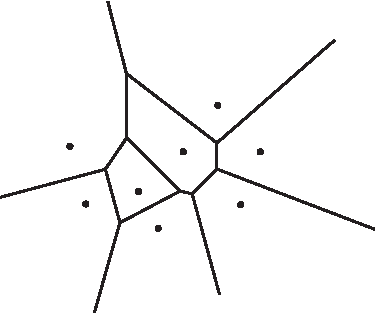
\includegraphics[width=0.3\columnwidth]{figs/voronoi}
\end{center}
\caption[Voronoi tesselation]{Decomposition of a metric space into different parts.
Every point in the plane is categorized based on which
centroid (black dots) it is closest leading to subsets of
points where all points are closest to a particular centroid (Figure adapted from 
\citealt{aurenhammer1991voronoi}\oldindex{Aurenhammer, F.}).}
\label{f:voronoi}
\end{figure}

\subsection{Strict category membership}
Implementing such a notion of categorization has a profound 
impact on the processing of semantic structure. Instead of computing 
similarities and adding them to objects as in the lenient approach, categorization 
is implemented as a set of filter-operations which take some input set and filter the 
objects in the input set given a particular category which results in an 
output set only containing objects that are closest to that category (see 
\figref{f:filtering-operations} for an example of semantic structure with 
filtering operations). When evaluating a semantic structure
consisting of such filter operations, the set of objects in the context progressively
shrinks by applying subsequent filtering operations until one object is left, 
the topic or target of the semantic structure. For example, 
in the semantic structure shown in \figref{f:filtering-operations}, first
{\footnotesize\tt get-context} will introduce the set of objects perceived by
the robot, followed by the filtering of blocks, which results in the
set of blocks of the context. Afterwards, 
{\footnotesize\tt filter-by-spatial-category-group-based} will compute the centroid
of the group-based landmark, followed by the application of the 
spatial category {\footnotesize\tt left} to that landmark, which results in the
filtered set of ``left blocks''. The selector {\footnotesize\tt unique} only
checks whether the set of ``left blocks'' only contains one
object and if that is the case outputs that object.

This way of modeling semantic structure bears some similarities with
logic based approaches to semantics where, for instance, noun phrases denote a 
property that can be represented as a function from entities to truth 
values (see for example \citealt{barwise1981generalized}\oldindex{Cooper, R.}\oldindex{Barwise, J.}) -- in other words, where noun phrases denote sets of objects for which
the property holds. For instance the interpretation of \textit{Ball} (`ball') denotes 
the set of all balls in the context which is the same as filtering the context
for the set of balls. Such approaches are the dominant way of semantic
analysis for instance in generative grammar and they are also applied 
by many scholars to the semantic analysis of spatial language (see 
\citealt{eschenbach1997axiomatic}\oldindex{Eschenbach, C.}\oldindex{Kulik, L.} for an example). Consequently
one is tempted to take such an approach to modeling the semantics
of spatial language. However, there are some considerable problems
associated with the category membership approach particularly when 
facing the problem of \textsc{perceptual deviation}.\is{perceptual deviation}

\begin{figure}
\begin{center}
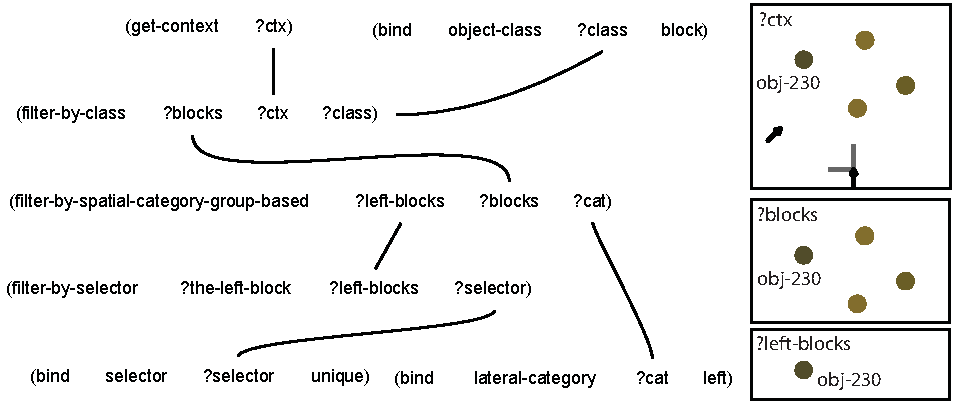
\includegraphics[width=.8\columnwidth]{figs/semantic-structure-filtering-der-linke-block}
\end{center}
\caption[Category membership semantics]{On the left side, the semantic structure of the phrase 
\textit{der linke Block} (`the left block') with {\footnotesize\tt filter} operations is shown. The images to 
the right show the progressive filtering of the set of objects in the context when the 
semantic structure is evaluated. The context {\footnotesize\tt ?ctx} contains all objects
perceived by the robot, whereas the set {\footnotesize\tt ?blocks} contains all blocks
filtered from the context and, finally, the set {\footnotesize\tt ?left-blocks} 
only consists of the object {\footnotesize\tt obj-230}.}
\label{f:filtering-operations}
\end{figure}

\begin{figure}
\begin{center}
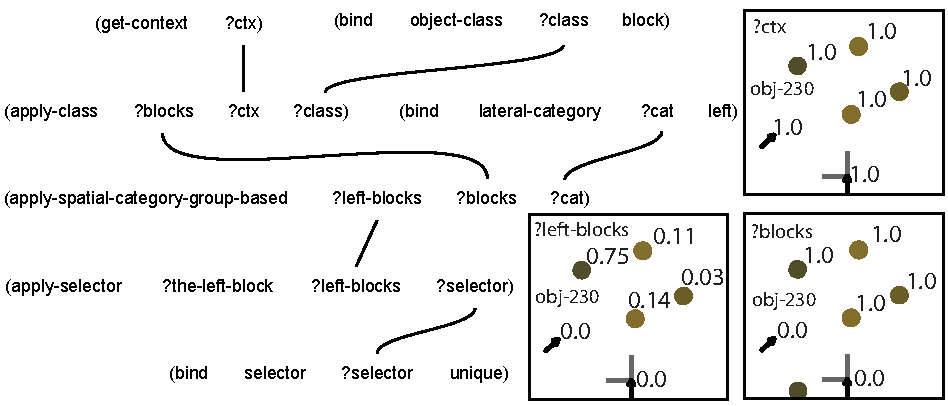
\includegraphics[width=.8\columnwidth]{figs/semantic-structure-apply-der-linke-block}
\end{center}
\caption[Lenient categorization semantics]{\is{categorization!lenient}%
On the left side, the semantic structure of the phrase
\textit{der linke Block} (`the left block') with {\footnotesize\tt apply} operations is shown. The images to
the right show the application of semantic operations which leads to the
bindings of the variables {\footnotesize\tt ?ctx}, {\footnotesize\tt ?blocks} and {\footnotesize\tt ?left-blocks}
with progressively changing similarity scores. For this example similarities are
multiplied. First the operation {\footnotesize\tt apply-class} is evaluated leading to
scores of for all entities of type block and
for all others. Next the spatial operation {\footnotesize\tt apply-spatial-category-group-based}, 
which computes spatial similarities based on a landmark is executed.
Consequently all objects in the {\footnotesize\tt ?left-block} entity set are scored with
indeed the left block object {\footnotesize\tt obj-230} having the highest
overall score.}
\label{f:apply-operations}
\end{figure}

While the target entity of the semantic structure in \figref{f:filtering-operations} 
is essentially the same as, for instance, for a comparable structure using the 
approach advocated in this book (see \figref{f:apply-operations}),
in many cases the category membership 
approach is bound to fail due to noise and uncertainty in the 
estimation of spatial distances and angles or other perceptual
data channels such as color. The problem is that no two robots perceive
the world in the same way. Colors, sizes, distances and 
angles are all estimated using
complicated visual processing which is subject to noise and uncertainty, which
makes for instance the distance of one object to another appear smaller
for one of the robots in the scene. For instance, in \figref{f:space-scene-2}
object {\footnotesize\tt obj-266} (which is object {\footnotesize\tt obj-253} in the world model 
of the hearer) is smaller and more to the right of the box, than in the world model
constructed by the hearer. In the case of strict category membership these
sorts of perceptual deviations can lead to problems in interpretation.
Even if grammar would allow for perfect transmission of a semantic structure,
in other words, even if there would be no ambiguity or problems
in linking when parsing a phrase like \textit{der Block rechts der Kiste}, the
evaluation of the underlying semantic structure can lead to misunderstanding, 
i.e. both robots think that the utterance is about different objects. 
The reason for this type of misunderstanding is the strict filtering of sets
underlying interpretation of phrases in the category membership
approach. While for the speaker the object in question, for instance 
{\footnotesize\tt obj-266} is still to the right of the box, this might not necessarily 
be true in the world model of the hearer, which can lead to no or false 
interpretations of the semantic structure. Consider 
\figref{f:perceptual-deviation}, where object {\footnotesize\tt obj-212}
for the speaker is to the intrinsic left of the box, whereas it is to the
intrinsic right for the hearer. Small estimation errors in judging
distance and angle can thus lead to very different categorizations of 
the same object.

\begin{figure}
\begin{center}
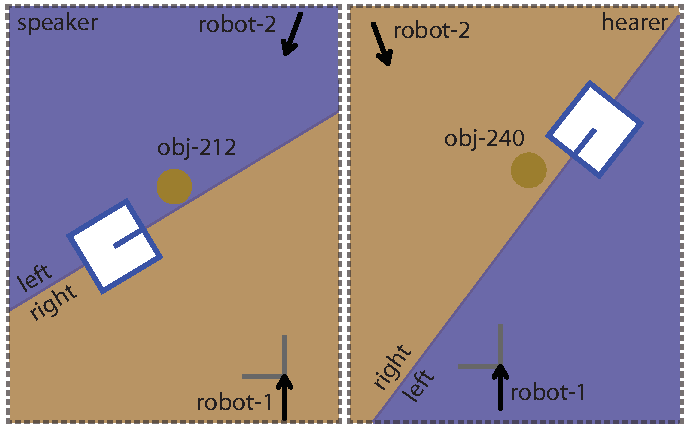
\includegraphics[width=0.5\columnwidth]{figs/perceptual-deviation}
\end{center}
\caption[Perceptual deviation]{Example for perceptual deviation and
impact on filtering operations}
\label{f:perceptual-deviation}
\end{figure}

\subsection{Lenient approach}
In contrast to the strict category membership, the approach 
advocated in this book does not rely on category membership, 
but only considers similarities to categories without enforcing the strict
membership criteria. In other words an object does not have to be closest
to the category {\footnotesize\tt left} in order to be categorized as left. Only one 
thing is important: the object needs to have a bigger similarity with 
{\footnotesize\tt left} than any other object in the context (see Figure 
\ref{f:apply-operations} which shows the accumulation of scores).
From this fact alone one can predict that the lenient approach
is better suited for dealing with perceptual deviation, as it is less 
restrictive in interpretation. But another prediction can be made as
well. The approach is also less restrictive in conceptualization,
in the sense that the strict category membership constraint is
also not applied in finding a category to discriminate an object.
Consequently, the lenient approach should also be able 
to find semantic structure in cases where the strict membership
approach fails as its membership constraint cannot be met.

\begin{figure}
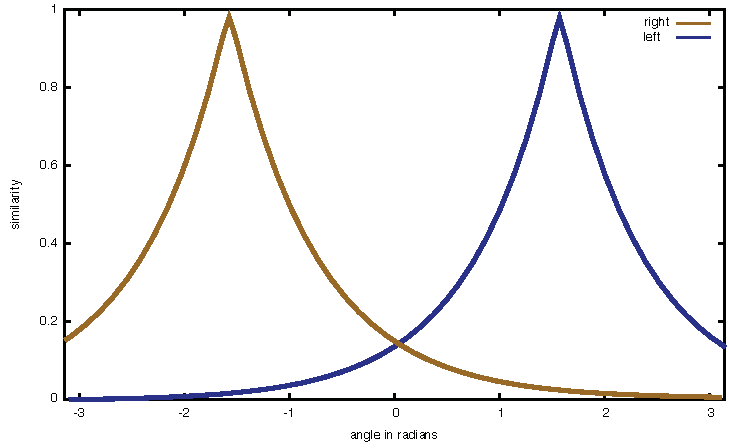
\includegraphics[width=0.6\columnwidth]{figs/lenient-vs-strict-interpretation}\\
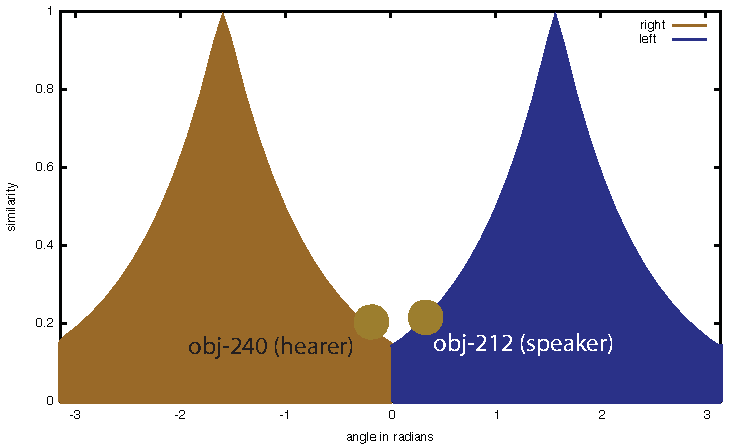
\includegraphics[width=0.6\columnwidth]{figs/lenient-vs-strict-interpretation-strict}\\
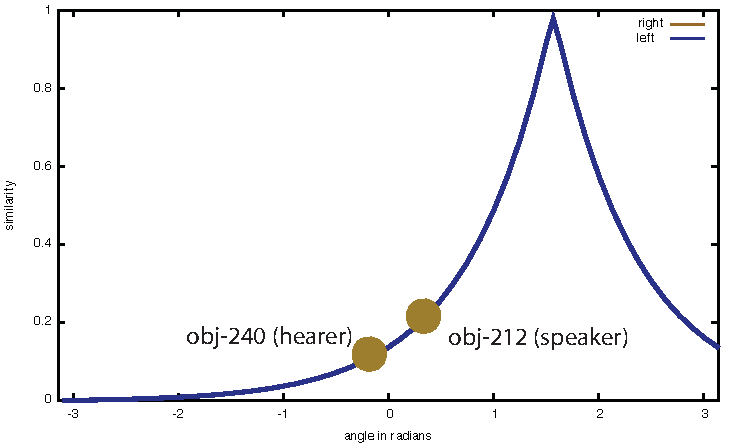
\includegraphics[width=0.6\columnwidth]{figs/lenient-vs-strict-interpretation-lenient}
\caption[Lenient vs strict categorization]{\is{categorization!strict}%
Lenient versus strict categorization\is{categorization!strict}.
The first figure shows 
the similarity functions for {\footnotesize\tt left} and {\footnotesize\tt right} 
categories over the angle. The second figure shows the decomposition
of the angular space using the strict approach. The third figure shows
how the lenient approach uses the similarity function of the spatial category
to retrieve the correct object.}
\label{f:lenient-vs-strict}
\end{figure}

Figure \ref {f:lenient-vs-strict} contrasts the example in Figure \ref{f:perceptual-deviation} 
from the viewpoint of strict and lenient discrimination. The top figure shows 
the similarity functions for {\footnotesize\tt left} and {\footnotesize\tt right} categories over the angle, 
from which the decomposition of the angular space show in the middle Figure follows.
The particular similarity function of the two categories interact in the decomposition
of the space. Object {\footnotesize\tt obj-212} is categorized by the speaker as being to the
left, whereas the same object for the hearer which he knows as object {\footnotesize\tt obj-240} is 
to the right. When the speaker thus conceptualizes the object as left, the hearer has no 
chance of retrieving the object in the strict interpretation case. On the other hand, when
applying a lenient discrimination scheme (bottom figure) there is no interaction 
between the categories {\footnotesize\tt left} and {\footnotesize\tt right}.
The decision whether or not the hearer is able to discriminate the correct object
depends on whether object {\footnotesize\tt obj-240} is indeed the most similar object
to the category {\footnotesize\tt left} (which it is in this case). To ensure that agents
can always find the correct object, category similarity functions always
span across the complete space. For instance, for the angular category
{\footnotesize\tt left} every angle has a similarity bigger than zero. For some angles
similarity is small, but importantly it is never below zero.

\subsection{Experimental setup}
We can study the difference of the two approaches systematically by letting agents
interact in controlled spatial scenes and see
which of the two approaches performs better in a discrimination task. 
In order to to study only the effect of the particular implementation of semantic 
operations, I eliminate the influence of language using 
direct meaning transfer, in which the hearer is passed the
semantic structure conceptualized by the speaker without going
through production and parsing of syntactic structure. 
This is equivalent to having 
a language where sufficient information is provided in each utterance
to decode the semantic structure intended by the speaker 
without uncertainty, ambiguity or loss of information.
The particular interaction script used in the experimental
setup is the following. Always two agents from a population interact. 
One is the speaker, the other the hearer. The speaker perceives the world,
picks a topic and tries to conceptualize a semantic structure
for reaching his communicative goal. If he is successful in finding
semantic structure for discriminating the topic, he passes the semantic
structure to the hearer. The hearer interprets the semantic structure
by simply evaluating it. Afterwards he points to the object he
thinks the semantic structure was about. 

Thus, there are four different outcomes of the game.
\begin{description}
\item[Conceptualization failed] After the speaker choose a topic, he has
to conceptualize a semantic structure that discriminates the topic.
This process fails, if the speaker cannot find any semantic structure
that allows him to discriminate the object from all other objects in the
context.
\item[Interpretation failed] After the speaker successfully conceptualized
a discriminating semantic structure, the hearer interprets this structure
by simply evaluating the semantic program. If this evaluation
yields no result, the hearer is said to have failed.
\item[Pointing failed] When the hearer successfully interpreted the
semantic structure passed to him by the speaker, he points
to the topic he interpreted. The speaker then interprets whether
the object pointed to is indeed the topic. If this is not the
case then pointing failed.
\item[Success] The hearer pointed to the correct object and
the game is a success. 
\end{description}

We can compare the two approaches to categorization 
using two different sets of agents --
one in which agents are equipped with a lenient implementation 
of semantic operations as advocated in this book, and a second where
agents are equipped with category membership based
semantic operations. Both agents were equipped with
complex semantic structure, which allowed them to use
group-based reference, landmarks, relative and intrinsic frames
of reference together with proximal and projective spatial categories
implemented as in the German space semantics discussed in 
\chapref{s:german-space-semantics}. I test both populations and 
their respective success and failure on different sets of spatial scenes.

\begin{figure}
\begin{center}
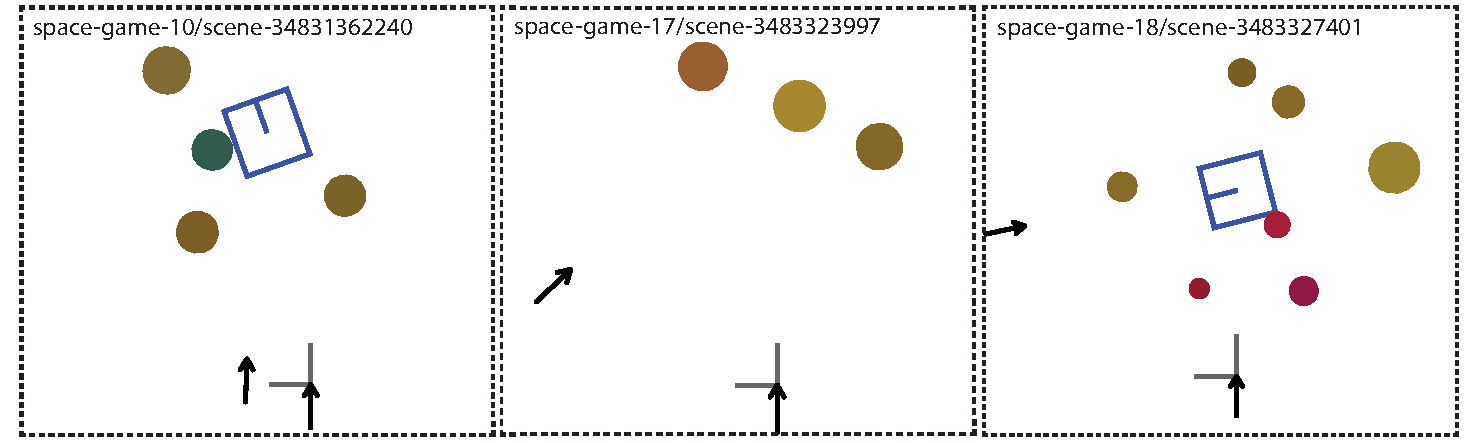
\includegraphics[width=.8\columnwidth]{figs/apply-filter-comparison-scenes}
\end{center}
\caption[Spatial scenes used to compare lenient vs. strict categorization]
{\is{categorization!strict}\is{categorization!lenient}%
This figure exemplarily shows spatial scenes used for comparing lenient and strict
categorization implementations. The left image shows an example scene from the data 
set labeled {\footnotesize\tt space-game-10} which consists of scenes with one landmark and two robots 
that can be used as reference systems. Spatial scenes in data set {\footnotesize\tt space-game-17} (middle image) consist of scenes without boxes.
Only the two robots and group-based reference are available for conceptualizing the spatial
scene. The right image shows an example from data set {\footnotesize\tt space-game-18} which features a box 
just as {\footnotesize\tt space-game-10}, but in much more complex spatial layouts.}
\label{f:lenient-vs-strict-scenes}
\end{figure}

\subsection{Results}
The results in \figref{f:apply-filter-comparison} show
a clear advantage for the lenient approach proposed in this 
book. The success in interaction for this approach to 
spatial categorization is consistently above 85\% across various 
spatial scenes, whereas the success of strict categorization\is{categorization!strict} drops to 22\%
in the worst case ({\footnotesize\tt space-game-18}) but consistently performs below 60\%
success showing the power of the lenient approach to deal even with 
very complex spatial scenes (see \figref{f:lenient-vs-strict-scenes} for
some example scenes from the different spatial scenes). Notably,
the lenient approach in almost all scenes is able to successfully conceptualize
the spatial scene for the topic in question. Only few cases in data set {\footnotesize\tt space-game-18}
are marked for failure in conceptualization. On the other hand, the strict
approach shows enormous problems even conceptualizing for particular
objects in particular scenes. Almost all cases of failure are either due to 
failures of conceptualization or failures of interpretation, where conceptualization
as can be seen takes the major blame for failure.

\begin{figure}
\begin{center}
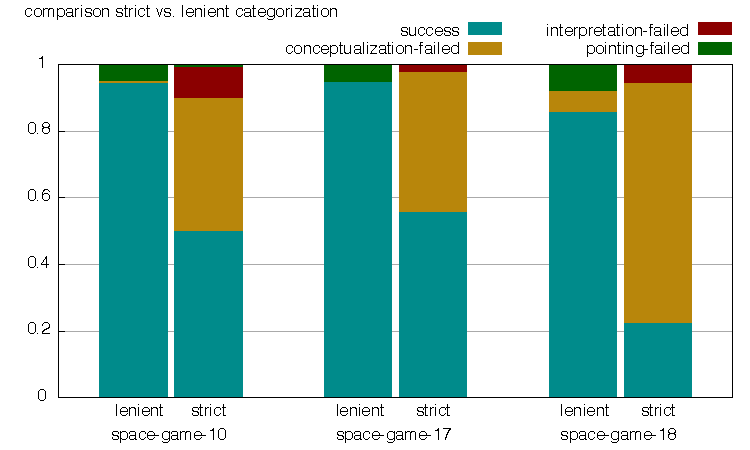
\includegraphics[width=.8\columnwidth]{figs/apply-filter-comparison}
\end{center}
\caption[Comparison of filter type semantics and apply semantics]
{Results of comparing strict versus lenient categorization\is{categorization!lenient}
on different sets of spatial scenes}
\label{f:apply-filter-comparison}
\end{figure}
% [todo: add condition names and svg's]

Failures to conceptualize in the case of strict category membership are caused by 
insufficient clustering of the input space. The problem is that categories are not
dense enough to allow the speaker to conceptualize for the particular topic.
Failures to interpret on the other hand are caused by perceptual deviation.
Strikingly, there are no interpretation failures in the case of the lenient approach
highlighting its power to deal with perceptual deviation. Maybe for the strict
approach the problem could be eased. For instance one could increase
the number of possible decompositions of the sensorimotor space
by adding more categories which allows the speaker to more easily conceptualize.
\figref{f:filter-increased-categories} shows the effect of 
adding more categories to the inventory of strict categorization\is{categorization!strict} agents.
It compares four conditions (over the different spatial scenes):
``german'', ``double'', ``triple'' and ``quadruple''.
``German'' refers to the set of categories introduced earlier, e.g. front, back, left, 
right and so forth. ``Double'' refers to a set of categories where the number of 
categories is doubled. So for instance, instead of two lateral categories left and right 
there are now four. The same holds for frontal and proximal categories. In the ``triple'' 
condition agents are equipped with three times as many categories and in the
``quadruple'' condition the number of categories is four times compared to the 
german condition. 

In some cases most notably for data set {\footnotesize\tt space-game-18} 
more categories indeed helps triple the success in interaction. This is not all that
surprising in the sense that there was a lot of room for improvement in the 
first place. For the other two sets of scenes success in interaction stays 
pretty much the same. And it seems that also for {\footnotesize\tt space-game-18} a certain
limit of improvement is reached, as success actually drops again for quadrupled
number of categories\is{measures!number of categories}. The most interesting point is, however, that overall 
success in interaction stays roughly the same for most spatial scenes 
and failures of the speaker to conceptualize
are replaced by the inability of hearers to interpret. This is most strikingly the case
in condition {\footnotesize\tt space-game-17} where this type of error accounts for 20\% of all
interactions and half of the unsuccessful ones. In other words, the more categories 
there are available, the more impact perceptual deviation has on the strict set approach.
The reason for this can be found in the interaction of categories that determines 
the decomposition of the space. The more categories there are, the smaller the 
area of applicability of categories
becomes, and consequently the more likely it becomes that an object that is
categorized as belonging to a certain category by the speaker will be 
categorized differently by the hearer. One might
wonder what the effect of more categories is on the lenient categorization\is{categorization!lenient}
approach. \figref{f:apply-increased-categories} shows that while there
is some impact of more categories in the difficult scenes of data set
{\footnotesize\tt space-game-18}, overall there is no significant increase in success in
interaction.

\begin{figure}
	\begin{center}
		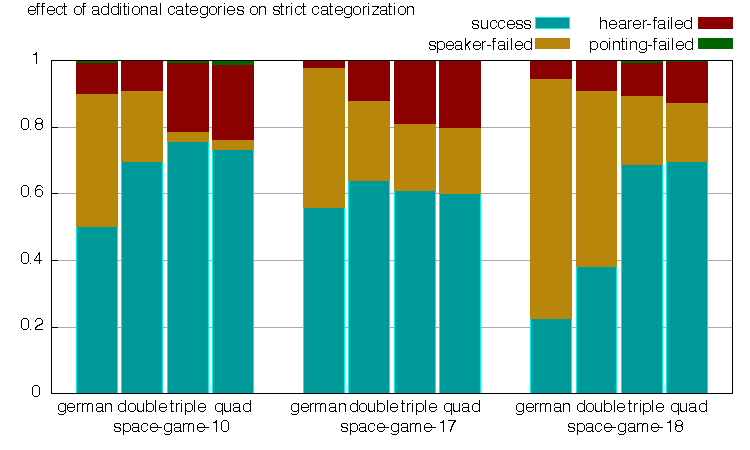
\includegraphics[width=.8\columnwidth]{figs/filter-more-categories.pdf}
	\end{center}
	\caption[Effect of additional categories on strict categorization]
	{Results of comparing different sets of spatial categories and their 
		effect on the strict categorization\is{categorization!strict} approach}
	\label{f:filter-increased-categories}
\end{figure}
\begin{figure}
	\begin{center}
		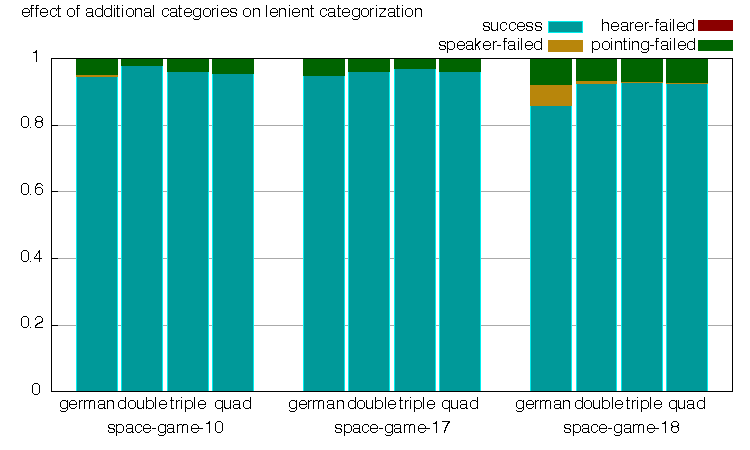
\includegraphics[width=.8\columnwidth]{figs/apply-more-categories.pdf}
	\end{center}
	\caption[Effect of additional categories on lenient categorization]
	{Results of comparing different sets of spatial categories and their 
		effect on the lenient categorization approach.\is{categorization!lenient}}
	\label{f:apply-increased-categories}
\end{figure}

%%%%%%%%%%%%%%%%%%%%%%%%%%%%%%%%%%%%
\section{Summary}
We can conclude that the communicative intentions of an agent influence
how spatial scenes are conceptualized, i.e. which spatial relation is chosen, 
which frame of reference, or which landmark. The most important
factor is whether an agent wants to discriminate or describe an object.
But, preferences for particular spatial relations, perspective or frames of 
reference are also important. This chapter showed that these factors
are easily operationalized using IRL. Experimental results demonstrate that the system
is powerful enough to enable robotic agents to reliably conceptualize 
spatial reality. The results of this chapter are further discussed in \cite{pauw2010embodied,pauw2012embodied,spranger2012deviation}.\oldindex{Spranger, M.}\oldindex{Pauw, S.}



% \bibliographystyle{diss}
% \bibliography{papers,space}
% \end{document}
